\documentclass{article}
\usepackage[dblblindworkshop]{neurips_2026}
\workshoptitle{Foundation Models for Temporal Systems (FMTS): From Forecasting to World Modeling}
\usepackage{fontspec,xeCJK}
\setCJKmainfont[BoldFont=SimHei,ItalicFont=KaiTi]{SimSun}
\setCJKsansfont{Microsoft YaHei}
\setCJKmonofont{Microsoft YaHei}
\usepackage{hyperref,url,booktabs,amsmath,amsfonts,microtype,graphicx}
\usepackage{etoolbox}
\patchcmd{\abstract}{Abstract}{摘要}{}{}
\hypersetup{hidelinks,pdfauthor={},pdftitle={当准确预测还不够：物理结构热过程世界模型}}
\newcommand{\degc}{\ensuremath{^{\circ}\mathrm{C}}}
\renewcommand{\abstractname}{摘要}
\renewcommand{\refname}{参考文献}
\renewcommand{\figurename}{图}
\renewcommand{\tablename}{表}
\title{当准确预测还不够：\\物理结构热过程世界模型}
\author{Anonymous}
\begin{document}
\maketitle

\begin{abstract}
在一台在役 600\,MW 直流炉上开发预测前馈时，我们发现一个实际问题：准确的主汽温预测不一定能描述改变减温阀的后果。为此，我们构建物理结构热过程世界模型，由物理动力学承载动作通道，由历史观察器和有界神经热功率修正补充不完整的状态与动力学。在共享的内部验证窗口上，三种子比较得到 180 秒内累计主汽温 MAE：纯黑箱为 0.371\degc{}，纯灰箱为 0.969\degc{}，GRU 融合模型为 0.443\degc{}。融合模型相对黑箱付出 0.0725\degc{}（19.6\%）的预测误差代价；其双阀响应呈明显负向，而黑箱在注册诊断中几乎不敏感。采用 token 化与交叉注意力的观察器在三个种子上均未改善 MAE。这些结果量化的是预测代价与模型动作响应，不是现场响应保真或已验证的控制收益。
\end{abstract}

\section{工程问题：预测一个温度，不等于评估一个动作}

本研究起于一台已运行 12 年的 600\,MW 燃煤直流炉的预测前馈开发。工程开发中，温度预测器能够很好地拟合历史轨迹，但改变输入的减温阀位后，预测温度的响应可能很弱，或者方向不符合预期。这是作者提供的工程动机，不是一项已经量化的在线干预实验。其操作意义在于：预见温度偏离可以支持报警或扰动前馈；但如果用同一个模型比较不同的阀门修正，就需要它描述这些动作的后果。

闭环日志并不自动提供这种能力。阀门随温度和运行条件变化，预测器可能利用变量间的相关性，而没有获得独立有效的动作响应通道。闭环辨识研究早已区分这些问题~\cite{forssell1999closedloop}。受控世界模型的近期理论在限制性假设下，将转移可辨识性与条件动作激励联系起来~\cite{zhang2026identifiability}。我们仅以这一机制解释研究动机，不把线性高斯条件下的界限直接套用于非线性锅炉。

物理建模提供另一种归纳偏置，但不完整的边界条件、不可直接测量的热储能状态和未知扰动效应，使模型跨动态工况使用并不容易。Fan 型锅炉模型本身已将守恒关系与数据辨识项结合~\cite{fan2020thermal}，因此我们的出发点不是“传统物理模型普遍无效”。另一方面，主汽温预测精度~\cite{zhang2026sst}本身也不能回答动作响应是否可信。沿着混合动力学建模思路~\cite{rackauckas2020ude,yin2021aphynity}，本文提出的问题是：\emph{学习能否改善物理热过程模型，同时保留显式阀门通道；这种选择伴随多大的预测精度代价？}

我们构建一个共享物理转移，同时用于已记录动作下的预测和替代动作下的推演。贡献在于具体的学习位置设计：锚定的慢状态初始化与内部热功率修正，以及聚焦主汽温精度、两级减温阀响应的工业对照。预先规定的观察器比较最终保留 GRU，而不是为了形式新颖换用更复杂的 token 架构。本研究面向从预测走向动作条件世界模型的接口，不声称进行了基础模型预训练、跨电厂迁移或控制器部署验证。

\clearpage
\section{在物理动作通道内引入学习}\label{sec:method}

\begin{figure}[!ht]
\centering
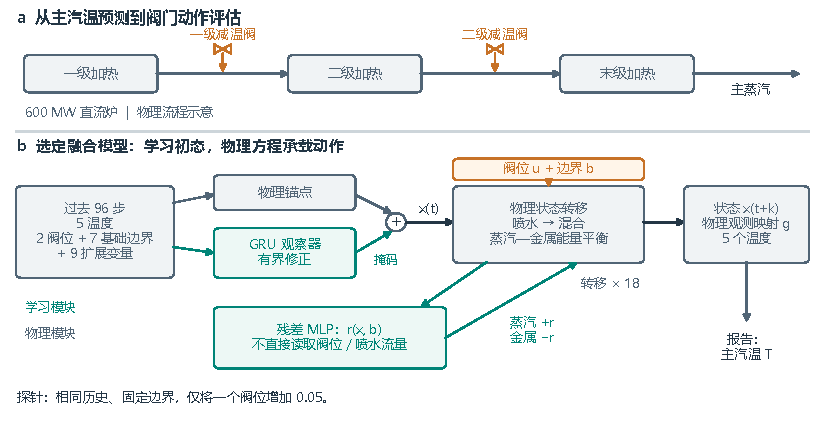
\includegraphics[width=\linewidth]{figures/fig1_architecture_zh.pdf}
\caption{\textbf{物理转移承载动作，神经模块补全模型。}选定融合模型使用只读历史的 GRU 与有界功率闭合项（绿色）。阀门驱动的喷水、输运、混合及蒸汽—金属能量平衡构成灰箱推演。闭合项不直接读取阀位或实测喷水总量，但读取已受动作影响的状态。预测与探针共享权重和初态。图中只画均值路径；该融合模型已消融再润湿。}
\label{fig:model}
\end{figure}

\paragraph{状态和输入。}
历史 $\mathcal H_t$ 包含以 10 秒采样的 96 步：5 个温度、2 个阀位、7 个基础边界和 9 个只读历史的扩展变量，共 23 维。11 维物理状态包括 3 个蒸汽焓、3 个金属温度、燃料滞后、2 个液体存量和 2 个喷水输运状态。阀位决定喷水流量，经输运和焓混合影响下游温度（图~\ref{fig:model}）。热力学观测映射输出五个温度，本轮只报告主汽温。

\paragraph{锚定初始化与热闭合项。}
五个观测温度不能确定所有物理状态。由观测关系形成稳态锚点 $x_{\rm anc}$，再由 GRU 提供有界修正：
\begin{align}
x_t &= x_{\rm anc}(\mathcal H_t)+M[0.1s_x\odot\tanh d_\phi(\mathcal H_t)],\label{eq:init}\\
r_k &= R\tanh f_\theta(x_k,b_{k+1}^{\rm allow}),\quad
x_{k+1}=\Phi_\psi(x_k,u_{k+1},b_{k+1};r_k),\label{eq:trans}\\
\hat y_{k+1}&=g_\psi(x_{k+1},b_{k+1}).\label{eq:obs}
\end{align}
$s_x$ 为固定状态尺度；$M$ 只选择金属温度和燃料滞后，保留快状态的锚定值。闭合项在每段蒸汽功率中加入 $r_j$，在金属功率中加入 $-r_j$，$R=30{,}000$\,kW。它们是内部功率修正，不是附加的温度预测头。转移使用可学习物理参数和 2 秒半隐式子步。两种融合候选的再润湿增益均固定在近零值；纯灰箱参考保留再润湿。

\paragraph{共享转移不等于保真保证。}
固定历史和边界后，诊断定义为 $\widehat{\Delta T}_{1:H}=\hat T(\mathcal H_t,u^+,b)-\hat T(\mathcal H_t,u^0,b)$。相同动作必须产生相同输出。闭合项不直接读取阀位和喷水总量，只限制这条直接捷径，并没有去除经状态传递的动作依赖；正负配对功率也不保证真实响应幅值。token 候选只将 GRU 观察器替换为变量—时间分块和状态查询交叉注意力，物理推演与闭合项不变（附录~\ref{app:implementation}）。

\clearpage
\section{聚焦且冻结的对照协议}\label{sec:protocol}

\paragraph{数据和共同评估。}
单个流程侧有 707,709 个样本，约 82 天，按时间以 75/15/10 划分。本轮仅使用内部验证集，最终测试段仍锁定。v0.2 在本轮训练前冻结，但此前验证实验已经参与设计。四个实验臂、种子 0--2 共享同一个抽样的 20,000 窗口训练库、256 个预测窗口和 64 个响应历史。两个评估集合均覆盖 13 个 UTC 日。合格条件由基础通道有效性、历史扩展变量有限且在注册范围内、严格 10 秒连续性共同决定，不按结果筛选窗口。

预测时给定未来 18 步的已记录阀位及 7 个基础边界，这是 \emph{oracle 条件预测}，不是未来边界未知时的前瞻预测。包括水煤比、负荷在内的 9 个扩展变量严格只读历史，归一化统计量只由训练行得到。累计主汽温 MAE 为
\begin{equation}
E_H=\frac{1}{3}\sum_{s=0}^2\frac{1}{|\mathcal D|}\sum_{d\in\mathcal D}
\frac{1}{n_d H}\sum_{i\in d}\sum_{h=1}^{H}|\hat T^{(s)}_{i,h}-T_{i,h}|.
\label{eq:metric}
\end{equation}
即先等权平均日，再等权平均种子；H18 是 10--180 秒的累计平均，不是只计算末端误差。

\begin{table}[!ht]
\centering\small
\begin{tabular}{lccc}
\toprule
方法 & H1 & H6 & H18\\
\midrule
持续值（共同参考） & $0.085$ & $0.268$ & $0.639$\\
纯黑箱（变量 token） & $0.100\pm0.013$ & $0.191\pm0.011$ & $0.371\pm0.007$\\
纯灰箱（稳态、无闭合项） & $0.224\pm0.003$ & $0.529\pm0.007$ & $0.969\pm0.008$\\
GRU 融合（选定） & $0.093\pm0.007$ & $0.224\pm0.014$ & $0.443\pm0.022$\\
Token 融合（候选） & $0.111\pm0.004$ & $0.306\pm0.019$ & $0.654\pm0.048$\\
\bottomrule
\end{tabular}
\caption{\textbf{v0.2 信息合同下的主汽温预测。}累计 MAE（\degc{}）：日均后取三种子均值 $\pm$ 样本标准差；持续值参考为共享的确定量。H1/H6/H18 对应 10/60/180 秒。结果来自固定预算与验证集选模，不是锁定测试估计。}
\label{tab:prediction}
\end{table}

\paragraph{完整方法比较，而非完全匹配的架构消融。}
纯黑箱借鉴 iTransformer 的变量 token 思路~\cite{liu2024itransformer}并增加未来协变量接口，不是对已发表主汽温模型的原样复现。它与两种融合观察器共享 23 维历史；灰箱没有学习观察器和闭合项，只消费物理子集。黑箱还消费未来实测喷水总量，动作驱动的物理转移则忽略该通道。结构模型使用五温度高斯 NLL（24,000 更新上限、batch 32），黑箱使用主汽温 MSE（3,000 更新、batch 128）。12 个运行均达到上限，报告验证 H18 MAE 最低的检查点。信息、损失、预算和再润湿差异意味着不能把跨模型族差异归因于某一个架构组件。

\paragraph{选择与响应协议。}
token 只有在三个配对种子中至少两个改善 H18 MAE、种子均值不高于 GRU 且满足实现门时才晋级，阀门响应不参与选择。响应探针将双阀和边界固定在历史末值，仅将一个阀位增加满开度的 0.05，上限为 1.0；本轮全部实际剂量在浮点精度内为 0.05。响应按日、种子等权平均。两个阀门的 64 个历史均通过注册的“历史范围加 0.05”检查；这一边际范围检查不等于条件动作激励或联合反事实支持。没有现场干预真值。

\clearpage
\section{结果：预测代价与模型动作响应}\label{sec:results}

\begin{figure}[!ht]
\centering
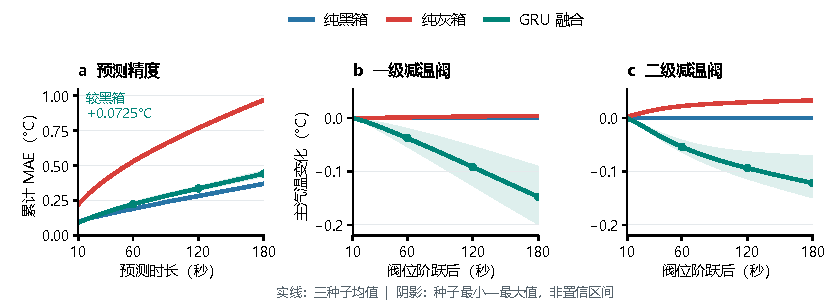
\includegraphics[width=\linewidth]{figures/fig2_prediction_response_zh.pdf}
\caption{\textbf{精度排序不能描述阀门响应曲线。}(a) 256 个共同窗口的累计主汽温 MAE。(b,c) 64 个共同历史上、固定边界、单阀增加 0.05 的“阶跃减基线”主汽温响应。实线先按日再按三种子平均；阴影是种子最小—最大值，不是置信区间。两张响应图共享刻度，保留所有注册窗口。这些是模型输出，不是实测现场增益。}
\label{fig:evidence}
\end{figure}

\paragraph{可以量化的精度代价，而非精度胜出。}
GRU 融合的 H18 MAE 为 0.443\degc{}，黑箱为 0.371\degc{}，差值为 +0.0725\degc{}（19.6\%）；相比灰箱的 0.969\degc{}，降低 54.3\%。排序取决于时长：GRU 的 H1 平均误差略低，但 H6 和 H18 更高（表~\ref{tab:prediction}）。配对日块区间中，GRU 相对黑箱的 H18 误差增量在两个种子上整体高于零，另一个种子区间含零。这是验证集选择后的描述性区间，不是经过选模校正的检验（附录~\ref{app:stats}）。

\paragraph{精度最好的预测器在该诊断中几乎不敏感。}
180 秒时，黑箱对一级、二级阀的种子平均响应约为 $+0.00010$ 和 $+0.00073$\degc{}；GRU 融合为 $-0.147$ 和 $-0.122$\degc{}，呈延迟发展的降温曲线（图~\ref{fig:evidence}）。两个阀门在三个种子上的 H18 响应均为负，六个末端日块区间均不含零。纯灰箱为 $+0.00448$ 和 $+0.03305$\degc{}：在这些拟合模型中，仅有物理状态表示也不保证预期的降温方向。但灰箱与融合的再润湿设置不同，不能把结果当作“神经组件修复方向”的隔离证明；没有实测现场增益时，也不能直接断言黑箱近零响应相对真值错了多少。

\paragraph{更复杂的观察器没有改善当前折中。}
token 的 H18 MAE 为 0.654\degc{}，比 GRU 高 47.7\%，每个种子均更差，未通过预定晋级规则；其均值也高于持续值参考的 0.639\degc{}。负向阀门响应不能推翻这一结果，因此保留 GRU。这是限定于该分块/查询观察器与预算的负结果，不是对 Transformer 的一般否定（附录~\ref{app:ablation}）。

\section{讨论与结论}
该世界模型将学习的热状态与功率修正放入显式、共享的物理动作通道。现有证据定位了一个候选折中：相对黑箱增加 0.0725\degc{} 预测误差，同时呈现非微弱的降温响应；它不是经校准的最优点，也不是 Pareto 前沿。oracle 信息和重复使用的验证集限制泛化结论，模型族之间的配置差异限制架构因果归因。匹配的 no-rewet 纯灰箱对照已单独注册，尚待执行；独立测试和现场响应校准仍未完成。对于需要评估动作的时序世界模型，应同时报告预测误差和动作响应；预测排行榜或物理结构本身，都不能证明模型已经适合决策。

\label{maintext:end}
\clearpage
\bibliographystyle{plainnat}
\bibliography{references}
\clearpage
\appendix
\section{实现与信息访问}\label{app:implementation}

\paragraph{物理模型。}
状态向量为 $(h_1,h_2,h_3,T_{m1},T_{m2},T_{m3},r_b,m_{\ell1},m_{\ell2},d_{sw1},d_{sw2})$。
温度—焓关系使用表格化 IAPWS 物性网格。观测映射读取物理状态和给定边界，没有独立的神经均值温度头。
稳态锚点由物理观测反演得到，融合模型只修正金属温度和燃料滞后；三个蒸汽焓、两个液体存量、两个喷水输运状态保留锚定初值。
均值修正幅度受固定状态尺度的 0.1 倍限制；观察器输出头零初始化时严格回到锚点。
每个 10 秒采样步由五个 2 秒子步组成。每个子步都用当前状态重新计算闭合项，式~\ref{eq:trans}省略了该内部组合。

\paragraph{闭合项的限制。}
两隐层 tanh MLP 输出三个分段有界功率修正。保守注入在蒸汽/金属两侧以正负配对形式加入。
输入是归一化物理状态和六个允许的基础边界，排除实测喷水总量。本轮没有额外潜变量或随机闭合项输入。
输入排除只是一项直接接口约束：状态本身已经受较早动作影响。令动作扰动下的状态灵敏度为 $S_k=\partial x_k/\partial\epsilon$，局部链式法则包含
\[
S_{k+1}=(\Phi_x+\Phi_r r_x)S_k+\Phi_u\,
\frac{\partial u_{k+1}}{\partial\epsilon},\qquad S_t=0.
\]
学习闭合项仍能通过状态修改灵敏度。正负功率注入限制残差作用位置，但不证明参数可辨识、所有工况下稳定或真实增益恢复。

\paragraph{观察器候选。}
两种观察器隐藏宽度均为 128。候选对 23 个历史变量分别以长度 16、步长 8 分块，每变量 11 块，共 253 个 token。
线性分块嵌入加变量和位置嵌入，经过一层四头 Transformer 编码器；11 个学习状态查询再交叉注意到其输出。
逐状态修正头同时读取查询特征与压力特征。GRU 和候选共享修正上界、状态掩码、物理转移、闭合项、历史扩展和种子对应的训练抽样。
token 不读取未来历史；它替换的是观察器，而不是以注意力端到端替换物理动力学。

\paragraph{黑箱。}
黑箱借鉴变量 token 预测~\cite{liu2024itransformer}：用 96 到 64 的线性映射嵌入每个历史变量，用独立的 18 到 64 映射嵌入每个未来通道（2 阀位、7 边界）。
32 个 token 经过两层四头 Transformer，再由展平线性头预测相对历史主汽温均值的 18 步偏差。dropout 为 0.1，前馈宽度 128。
这是本地适配基线，不是原始 benchmark 架构或物理引导主汽温模型~\cite{zhang2026sst}的原样复现。

\begin{table}[!ht]
\centering\small
\begin{tabular}{lrrrr}
\toprule
项目 & 黑箱 & 灰箱 & GRU 融合 & Token 融合\\
\midrule
消费历史扩展数 & 9 & 0 & 9 & 9\\
学习观察器 & --- & --- & GRU & 分块/查询\\
神经功率闭合项 & --- & 无 & 保守注入 & 保守注入\\
再润湿 & --- & 启用 & 消融 & 消融\\
接收梯度的参数数 & 111,250 & 99 & 65,808 & 278,248\\
更新上限 & 3,000 & 24,000 & 24,000 & 24,000\\
Batch size & 128 & 32 & 32 & 32\\
验证间隔（更新数） & 500 & 200 & 200 & 200\\
Patience（验证次数） & 3 & 20 & 20 & 20\\
\bottomrule
\end{tabular}
\caption{实际执行配置，而非容量/算力匹配 benchmark。活跃参数数排除已实例化但被旁路的网络；结构模型的观测不确定性参数可经 NLL 接收梯度。}
\end{table}

\section{数据合同、估计量和溯源}\label{app:stats}

7 个基础通道为蒸汽流量、给煤指令、分离器压力、分离器温度、给水温度、出口压力、喷水总量。
9 个扩展为修正燃料、投运磨煤机数、加权磨煤机气温、烟气氧量、总二次风、再热器 A/B 侧入口烟温、水煤比、机组负荷。
扩展只参与历史，不向任何模型提供未来扩展。水煤比在此是协变量，不是额外的物理功率修正；没有特征消融，不能分离其独立收益。

物理模型对基础通道使用固定工程尺度；扩展使用共同的训练行均值和标准差。黑箱所有历史通道使用训练统计量，输出以历史目标均值为偏置；给定未来基础协变量不经过该历史归一化。
未来喷水总量对黑箱可见，对动作驱动物理模型被忽略。阀位变化时保持这一通道不变，是诊断输入定义，不代表自洽的现场反事实。因此应按完整方法比较理解结果。

训练从固定的、带放回抽取的 20,000 窗口库中抽样。训练库、验证、响应 manifest 随机种子分别为 15,000、30,000、60,000。
训练种子控制初始化和后续 minibatch。所有模型的验证目标、时间标记和起点完全一致；所有探针共享起点、阀位剂量和支持域掩码。
256 个预测窗口、64 个响应历史均覆盖 13 个 UTC 日。窗口可以重叠，不将窗口视为独立实验单元。

每个种子的配对 H18 误差差值先在 UTC 日内平均，再对 13 个日均值带放回抽样 1,000 次，RNG 种子为 11,000，取 2.5/97.5 百分位区间。
响应曲线逐点采用相同流程。这些区间描述选定检查点条件下的日间变化，没有校正检查点选择、此前验证复用、多重比较或跨日序列依赖。
三个种子不是三台独立电厂；图中阴影则是三个种子的日均值最小—最大范围。

\begin{table}[!ht]
\centering\small
\begin{tabular}{lccc}
\toprule
H18 候选减参考（\degc{}） & 种子 0 & 种子 1 & 种子 2\\
\midrule
GRU $-$ 黑箱 & $0.068$ & $0.046$ & $0.104$\\
95\% 日块区间 & $[0.027,0.108]$ & $[-0.002,0.093]$ & $[0.067,0.137]$\\
GRU $-$ 灰箱 & $-0.537$ & $-0.541$ & $-0.500$\\
95\% 日块区间 & $[-0.784,-0.318]$ & $[-0.756,-0.341]$ & $[-0.725,-0.299]$\\
Token $-$ GRU & $0.267$ & $0.212$ & $0.154$\\
95\% 日块区间 & $[0.210,0.329]$ & $[0.155,0.269]$ & $[0.119,0.193]$\\
\bottomrule
\end{tabular}
\caption{从保存数组独立复算的配对描述性区间，不作经选择校正或确认性显著性声明。}
\end{table}

注册支持检查将每个阀位历史边际最小/最大值向外扩 0.05，并检查基线与干预序列。本轮两个阀门的 64 个历史全部通过，没有丢弃历史。
这个宽松的轴对齐检查不检验联合状态—动作支持、条件激励或保持边界不变的现实合理性；因此 supported-only 曲线与主曲线完全相同，不另画重复附图。

\paragraph{产物审计。}
回传包含 12 个检查点、训练 ledger 和 24 个预测/响应原始数组。本地只读审计验证产物哈希、检查点与输入身份绑定、共同索引配对。
独立数组归约检查代码指纹，重算每条预测曲线、响应曲线及配对区间，恢复相同融合模型选择。输入、映射、物性网格指纹保存在内部审计记录。
执行侧回传记录声称完成 24 组推理数组重放；本次写稿没有从原始现场记录独立再做推理重放。没有为初稿训练或访问 test。
审计确认回传证据的一致性，不确认未测量的现场干预响应真值。

\section{观察器选择与逐种子诊断}\label{app:ablation}

\begin{figure}[!ht]
\centering
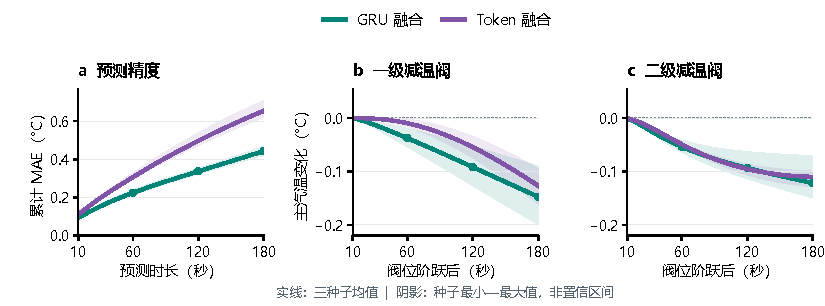
\includegraphics[width=\linewidth]{figures/figS1_observer_ablation_zh.pdf}
\caption{\textbf{Token 观察器不晋级。}物理配置、历史合同和评估 manifest 相同，仅观察器架构变化。三个种子的 token H18 预测误差均高于 GRU，两者均有负向平均末端响应；响应不参与选模。实线和阴影定义与图~\ref{fig:evidence}相同。}
\end{figure}

\begin{table}[!ht]
\centering\small
\begin{tabular}{lrrrr}
\toprule
方法 / 种子 & H18 MAE & 阀 1 H18 & 阀 2 H18 & 最佳更新\\
\midrule
纯黑箱 / 0 & 0.3735 & $+0.000013$ & $+0.001335$ & 3,000 \\
纯黑箱 / 1 & 0.3756 & $-0.000025$ & $+0.000678$ & 2,500 \\
纯黑箱 / 2 & 0.3628 & $+0.000305$ & $+0.000183$ & 3,000 \\
纯灰箱 / 0 & 0.9787 & $+0.004601$ & $+0.032581$ & 23,800 \\
纯灰箱 / 1 & 0.9623 & $+0.004401$ & $+0.033384$ & 24,000 \\
纯灰箱 / 2 & 0.9668 & $+0.004435$ & $+0.033175$ & 24,000 \\
GRU 融合 / 0 & 0.4414 & $-0.198801$ & $-0.145255$ & 21,000 \\
GRU 融合 / 1 & 0.4216 & $-0.090115$ & $-0.070247$ & 23,600 \\
GRU 融合 / 2 & 0.4664 & $-0.152901$ & $-0.149205$ & 21,000 \\
Token 融合 / 0 & 0.7086 & $-0.161024$ & $-0.099171$ & 23,800 \\
Token 融合 / 1 & 0.6340 & $-0.094119$ & $-0.128567$ & 23,600 \\
Token 融合 / 2 & 0.6203 & $-0.125057$ & $-0.102259$ & 22,000 \\
\bottomrule
\end{tabular}

\caption{逐种子的日均值，单位 \degc{}。预测为累计 H18 MAE；响应为 H18 末端差值，不是此前开发使用的末十步平均。全部运行达到预算上限。}
\end{table}

GRU 一级阀在种子 0/1/2 的末端区间分别为 $[-0.229,-0.167]$、$[-0.105,-0.075]$、$[-0.176,-0.128]$\degc{}；二级阀为 $[-0.168,-0.119]$、$[-0.083,-0.057]$、$[-0.172,-0.123]$\degc{}。
这些区间支持本探针定义下的负向模型响应。黑箱的微小差值接近大绝对温度预测的数值粒度，既不将其等同严格零，也不以它为分母宣称物理放大倍数。

\section{设计历程与尚未闭合的证据}

此前开发考察初态灵活性、残差位置、边界预测、再润湿诊断。它们使用不同输出聚合或信息合同，其 MAE 不与本轮主汽温单目标指标混合。
这些阶段提供锚定融合与无再润湿候选的设计依据，不是本轮的确认性重复实验。五温度平均与主汽温单目标平均不可互换，旧 H60 探针也不能扩张本轮注册的 180 秒证据范围。

剩余问题需要不同证据。选模后一次性锁定测试回答时间泛化，而不回答真实干预增益；匹配再润湿的灰箱对照才能更干净地分离加入观察器/闭合项的效果；独立校准的干预或适当辨识的自然实验回答现场响应幅值；未来边界由历史预测而非记录提供，才能评估前瞻使用。
看到本轮结果后，no-rewet 纯灰箱对照已按三种子和原预算单独注册，尚待执行；其他检查仍是提议，不是已完成结果，也不是对原协议的静默变更。

\paragraph{数据可用性与匿名。}
数据来自运行中的工业过程，原始记录的公开授权尚未建立，本稿不承诺公开原始数据。
数值图源、实验配置和审计记录已在本地保存；提交前需确认匿名共享材料和权限。正文、附录不包含私人仓库链接及现场身份。

\paragraph{语言模型辅助说明。}
语言模型工具辅助文章组织、翻译、绘图脚本开发和与保存结果的一致性检查，不替代现场响应测量。人类作者对最终科学主张、数值核验和投稿负责。

\end{document}
